\documentclass[11pt,a4paper]{article}
\usepackage[hyperref]{acl2020}
\usepackage{times}
\usepackage{latexsym}
\renewcommand{\UrlFont}{\ttfamily\small}

\usepackage{multirow}
\usepackage{booktabs}
\usepackage{graphicx}
\usepackage{amsmath}
\usepackage{xcolor}
\usepackage{tabularx}
\usepackage{float}
\usepackage{lscape}
\usepackage{rotating}
%\usepackage{geometry}
%\usepackage{pdfpages}
\graphicspath{ {./figs/} }
 
% This is not strictly necessary, and may be commented out,
% but it will improve the layout of the manuscript,
% and will typically save some space.
\usepackage{microtype}

\aclfinalcopy % Uncomment this line for the final submission
%\def\aclpaperid{***} %  Enter the acl Paper ID here

%\setlength\titlebox{5cm}
% You can expand the titlebox if you need extra space
% to show all the authors. Please do not make the titlebox
% smaller than 5cm (the original size); we will check this
% in the camera-ready version and ask you to change it back.

\newcommand\BibTeX{B\textsc{ib}\TeX}
\newcommand\todo[1]{\textcolor{red}{#1}}

\title{Multi-Task Patterns Training for Task Generalization}

\author{Asaf Maman \\
  Blavatnik School of Computer Science, Tel Aviv University \\
  \texttt{asafmaman@mail.tau.ac.il} \\}

\date{}

\begin{document}
\maketitle

\begin{abstract}
In recent years, appearance of large language models paved the way to prompt such model to extract predictions.
The idea behind this mechanism is to provide information about the task and use the model's general knowledge for a specific use.
This method appeard to be relatively successful and reveals many new options for potential use.
One approach for this subject is reformulating inputs as cloze-style phrases and leave one mask token to be used to derive classification prediction.
The restructured sequence and the tokens corresponding to each class label are called patten-verbalizer pair (PVP) and are used as task description.
Evaluating predictions this way enables us to use one language modeling head for multiple tasks with no need to initialize and train task specific weights.
In order to learn new task, the only change that needs to be done is chosing PVP for the new task. 
Multi-tasking training raises several question that I aim to answer in this project.
I found evidences that training models for multi-tasking, when done write, can be used without harming each task's performance.
In addition, when training on semantically similar tasks, multi-task training can, to some extent, generalize to unseen tasks.
\end{abstract}


\section{Introduction}

When handling classification tasks, the common method is to fine-tune the model together with a task-specific classification head.
One alternative way to deal with classification tasks is to reformulate the input examples as cloze-style phrases.
Each example is plugged into a fixed sentence structure, called \textit{pattern}, containing exactly one mask token.
The prediction is then determined according to scores the model assigns to a subset of tokens, called \textit{verbalizers}, each associated with one of the classes.
This mechanism reveals a few adventages over conventional classification methods.
First, it provides some sense of task description encoded in the \textit{pattern-verbalizer pair} (a.k.a. PVP).
This way the model gets information about the task and may be able to infer it from the PVP.
This can enable the model to adopt itself to new tasks without a need for large batch of new-task examples.

Another advantage is that training one language modeling head can be used for multiple tasks at once, without a need to train separate model for each.
Finally, making decisions using MLM predictions leverages the language modeling knowlaged attained during pre-training and use it for classification.

In this project I would like to investigate how masked language models performance are effected when trained on multiple classification tasks.
In addition, I would like to examine whether providing task description in the form of PVP can help MLMs generalize to \textit{unseen tasks}.
Finally, I will test these questions in few-shot setting using PET pipeline.


\begin{table*}[h]
	\centering
	\fontsize{9}{13}
	\selectfont
	\begin{tabular}{lcccccccccccccccc}
		\toprule
		& \textbf{agnews}    & \textbf{yahoo}    & \textbf{yelp-full}    & \textbf{yelp-polarity}    & \textbf{mnli}    & \textbf{qpp}    & \textbf{all}    & \textbf{unsup}    \\ \hline
		\textbf{agnews}        & 93.7   \tiny$\pm$ 0.06      & 81.7   \tiny$\pm$ 1.78      & 62.6      \tiny$\pm$ 6.10      & 62.7          \tiny$\pm$ 3.62      & 57.6 \tiny$\pm$ 5.06      & 63.9 \tiny$\pm$ 4.35      & 92.6 \tiny$\pm$ 0.45      & 66.7   \tiny$\pm$ 7.55      \\
		\textbf{yahoo}         & 56.1    \tiny$\pm$ 1.88      & 74.8   \tiny$\pm$ 0.25      & 39.3       \tiny$\pm$ 5.59      & 38.1           \tiny$\pm$ 7.25      & 24.4  \tiny$\pm$ 2.25      & 34.0 \tiny$\pm$ 5.39      & 74.1 \tiny$\pm$ 0.68      & 43.2   \tiny$\pm$ 7.66      \\
		\textbf{yelp-full}     & 27.9    \tiny$\pm$ 6.25      & 32.0   \tiny$\pm$ 2.23      & 67.7       \tiny$\pm$ 0.53      & 44.3           \tiny$\pm$ 3.94      & 34.1  \tiny$\pm$ 5.23      & 35.6 \tiny$\pm$ 13.9      & 66.6 \tiny$\pm$ 1.58      & 33.5   \tiny$\pm$ 11.6      \\
		\textbf{yelp-polarity} & 61.9    \tiny$\pm$ 10.4      & 59.6   \tiny$\pm$ 8.50      & 97.7       \tiny$\pm$ 0.26      & 97.7           \tiny$\pm$ 0.05      & 75.4  \tiny$\pm$ 4.52      & 75.5 \tiny$\pm$ 22.3      & 97.3 \tiny$\pm$ 0.29      & 67.3   \tiny$\pm$ 15.7      \\
		\textbf{mnli}          & 36.0    \tiny$\pm$ 1.31      & 35.6   \tiny$\pm$ 0.42      & 39.4       \tiny$\pm$ 9.67      & 42.1           \tiny$\pm$ 8.47      & 88.4  \tiny$\pm$ 0.07      & 51.8 \tiny$\pm$ 1.95      & 75.6 \tiny$\pm$ 16.3      & 38.4   \tiny$\pm$ 4.34      \\
		\textbf{qpp}           & 44.7    \tiny$\pm$ 14.5      & 43.7   \tiny$\pm$ 12.4      & 45.7       \tiny$\pm$ 15.2      & 41.1           \tiny$\pm$ 6.71      & 77.9  \tiny$\pm$ 0.74      & 85.9 \tiny$\pm$ 0.31      & 68.2 \tiny$\pm$ 27.7      & 43.9   \tiny$\pm$ 9.57      \\ \bottomrule
	\end{tabular}
	\caption{\textbf{Single-task training performence on all tasks}~---~reported accuracy results are averaged over all three possible patterns with standard deviation reported aside. Different training tasks are arranged in columns and evaluation tasks in rows. The "all" column corresponds to training on all tasks together and "unsup" column represents the unsupervised baseline without any pre-training.}\label{tab:single-on-train-set-summary}
\end{table*}






\section{Method}

\begin{figure}[b]
	\centering
	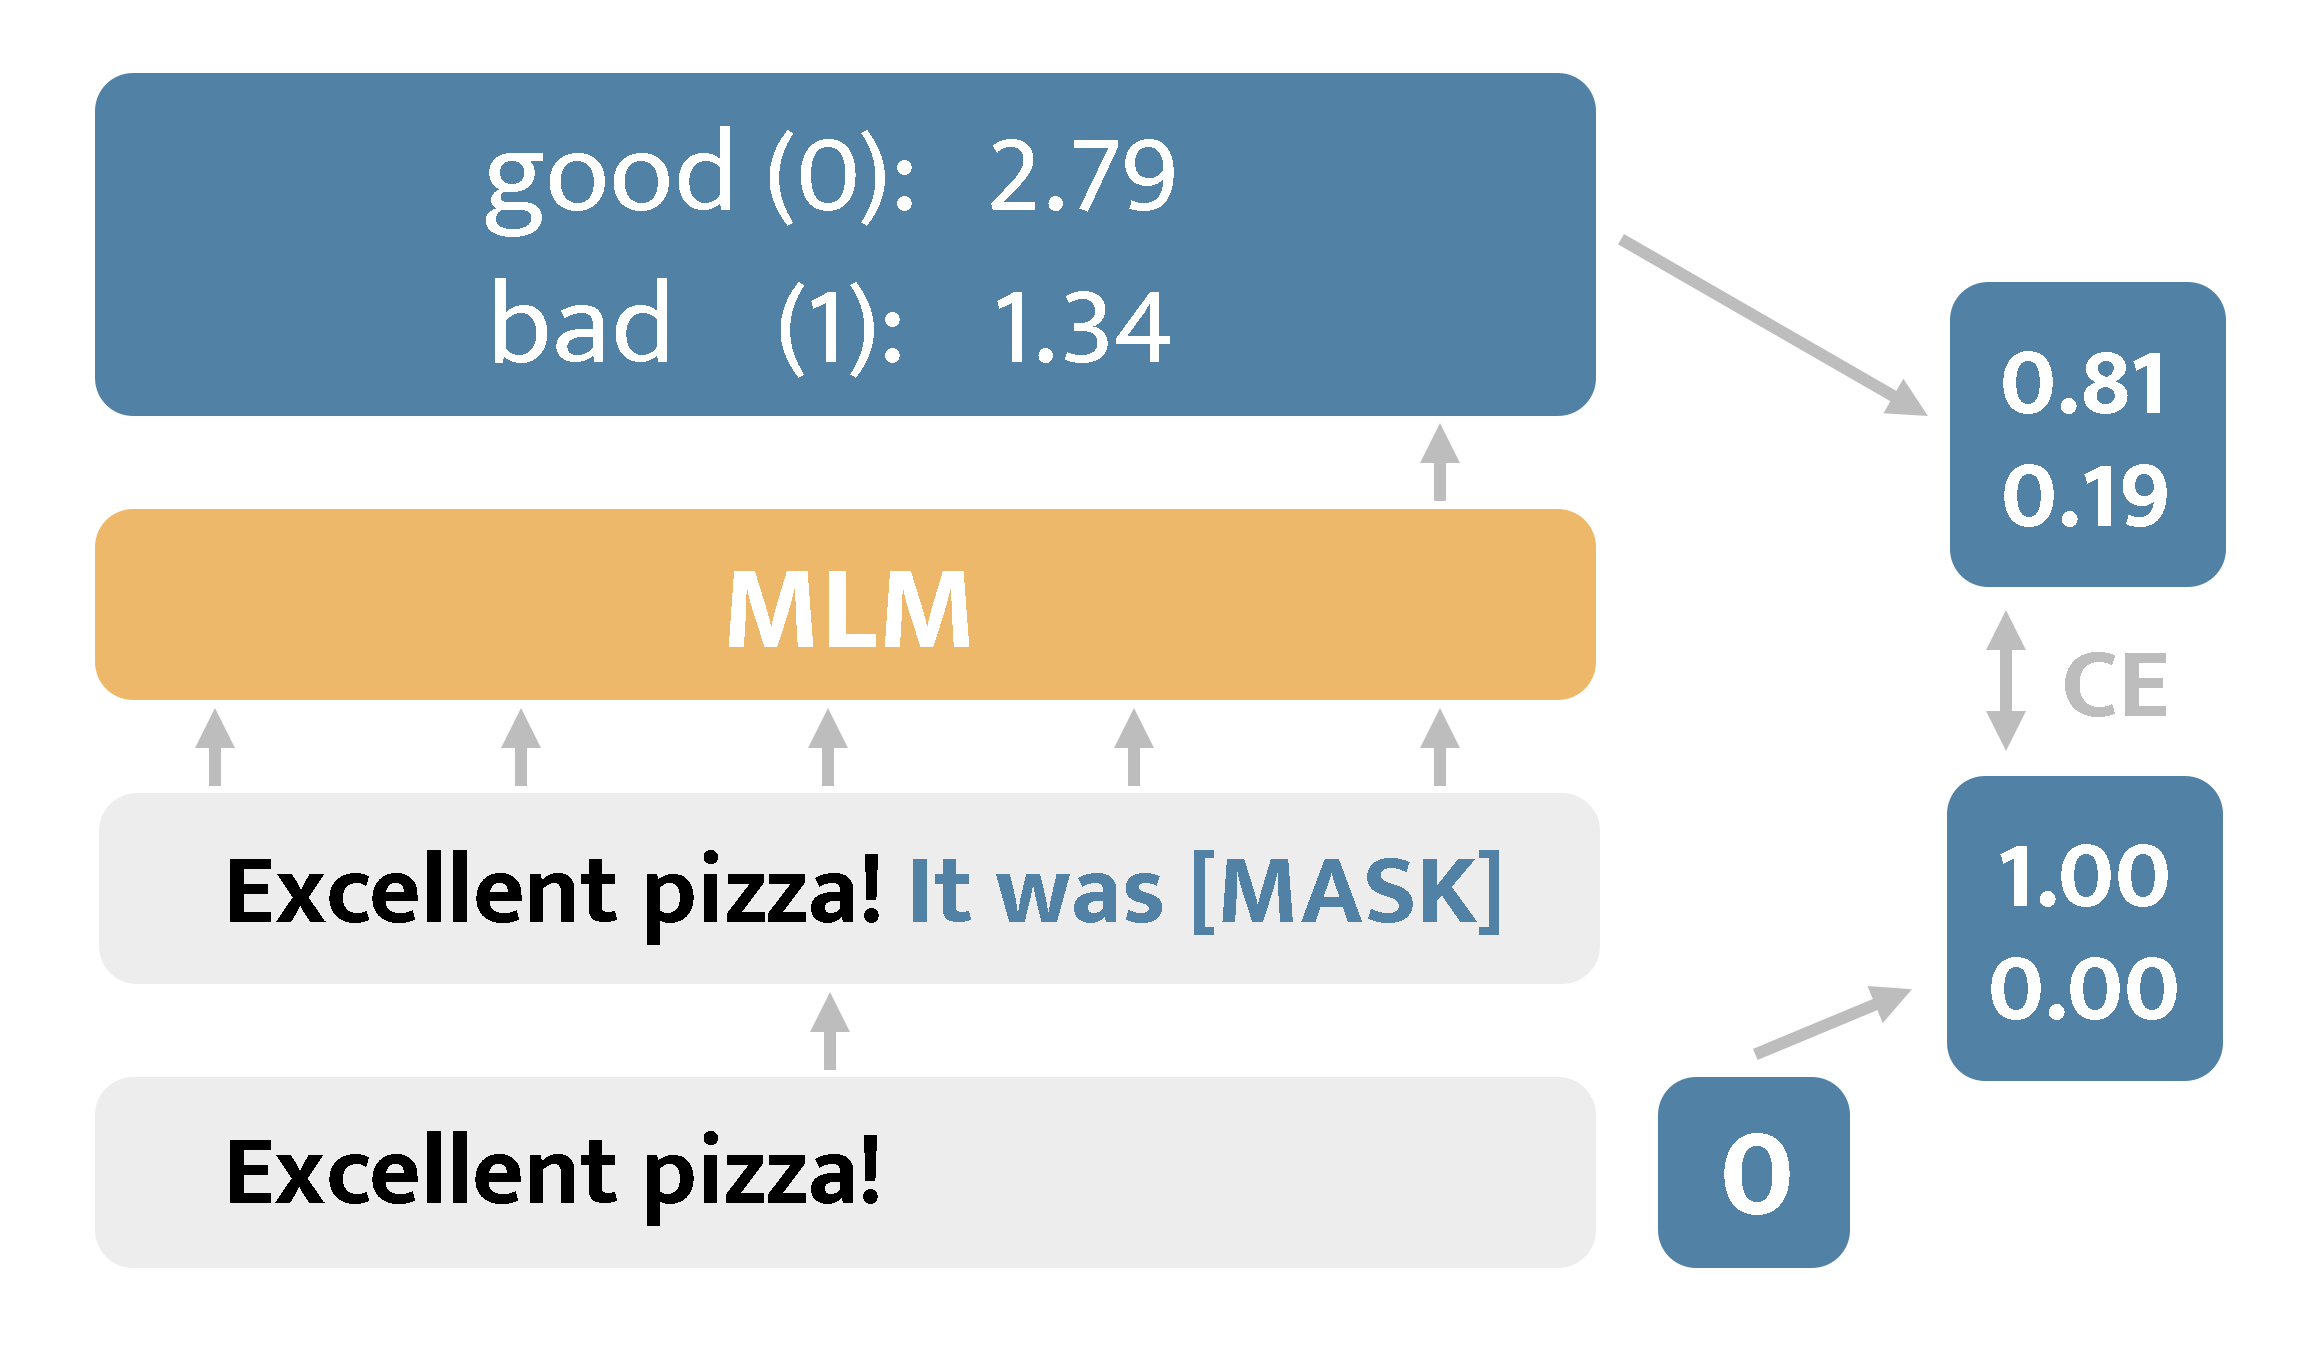
\includegraphics[width=\linewidth]{mlm_classification}
	\caption{Classification via prompting MLM with PVP}
	\label{normal_case}
\end{figure}

In general, using \textit{pattern-verbalizer pair} (PVP) can be formalized as follows: for a given masked language model $M$, vocabulary $V$ and set of labels $\mathcal{L}$, we define a pattern $P(\textbf{\text{x}})$ that takes as input the raw sample $\textbf{x}\in{}V^*$ and outputs a phrase $P(\textbf{x})\in{}V^*$ that contains exactly one mask token.
For each label in $\mathcal{L}$ we define the set of \textit{verbalizers} using the function $v:\mathcal{L}\rightarrow{}V$ that maps each label to a corresponding token.

We will apply the pattern $P(\textbf{x})$ on each input $\textbf{x}$ that we wish to evaluate.
Then we will use $M$ to process it and recieve the score it assigns to each token $t\in{}V$ at the masked token position.
We denote this unnormalized score as $M(t, \textbf{s})$.
Then we'll calculate the unnormalized score for each class label $l\in{}\mathcal{L}$, that is, $M(v(l) | P(\textbf{x}))$ and denote it by $s_{\text{\textbf{p}}}(l|\textbf{x})$ as the score our language model gives to class label $l$ providing with some PVP $\text{\textbf{p}}=(P, v)$.
Finally we normalize and calculate the probability distribution over the labels using softmax:
\[
	q_\text{\textbf{p}}(l|\textbf{x}) = \frac{e^{s_{\text{\textbf{p}}}(l|\textbf{x})}}{\sum_{l^{'}\in{}\mathcal{L}}e^{s_{\text{\textbf{p}}}(l^{'}|\textbf{x})}}
\]
We then use the cross-entropy between $q_\text{\textbf{p}}(l|\textbf{x})$ and the true one-hot encoded label to calculate the loss over all examples. 

We manually choose three PVPs for each task in a set of tasks $\{A_1, A_2, \dots, A_k\}$ and use them in the following experiments.



\section{Datasets}

I chose the following datasets to evaluate performence on.

\vspace{8pt}
\noindent \textbf{AG's News} \quad
A dataset for text categorization which contains 120K train samples and 7.6K test samples.
It contains articles formatted as title and text body.
The task is to classify the news to four categories: (1) World, (2) Sports, (3) Business, (4) Tech.

\vspace{8pt}
\noindent \textbf{Yahoo} \quad
Text categorization dataset. It contains 1.46M pairs of questions and answers.
The train set contains 1.4M samples and test set 60K samples.
The task is to classify each pair to its subject out of 10 possible options: (1) Society (2) Science (3) Health (4) Education (5) Computer (6) Sports (7) Business (8) Entertainment (9) Relationship (10) Politics.

\vspace{8pt}
\noindent \textbf{Yelp} \quad
Yelp Reviews dataset task is to classify a review for a 5-star rating.
It contains 650K train samples and 50K test samples.
There is another version for that task, while the 5-star scale named "Yelp Full", the second task is to predict whether the review sentiment was positive or negative.
The second task is named "Yelp Polarity".

\vspace{8pt}
\noindent \textbf{MNLI} \quad
The MNLI dataset contains pairs of sentences to classify between three possible NLI labels: (1) entailment (2) natural (3) contradiction. 
The dataset has 392K train and 9.8K test samples. 

\vspace{8pt}
\noindent \textbf{Quora Question Pairs} \quad
QQP contains 363K train samples and 40K test samples.
The task is to predict whether two sentences are paraphrases one of the other.

\subsection{Patterns}
The patterns for each task are presented in Appendix~\ref{apx:patterns}.


\section{Experiments}
\label{sec:experiments}

I conducted several experiments to test the questions raised above.
For each task, a set of PVPs was manually chosen, the PVP where taken from \citet{schick2020exploiting} for tasks that appear in their work.
For the additional tasks, the PVPs were chosen manually by human common sense. 

Each setting that will be described below was trained and evaluated on each PVP separatly.
To provide further analysis and possibly more insights about the behavior of the method, I evaluated each model not only on the PVP that it was trained on.

\subsection{Experimental Setup}
\label{sub-sec:experimental-setup}

All the additional implementation details and code can be found in this github repository\footnote{\url{https://github.com/asafmaman101/amnlp_final_project_code}}.

\subsection{Unsupervised Baselines}
To see how the fine-tuning influences each tasks performance, I evaluated as baseline the zero-shot performance of the pre-trained model with each PVP.

\subsection{Results}

\noindent\textbf{Single-task Training}\quad
Firsly, to see how our model perform on each task separatly, I trained and evaluated on single task.
The performance of supervised training using PVPs succeed to match the matching results with classification head showed in \citet{schick2020exploiting}.

In addition, when evaluating models trained on single task on different tasks, few of them showed improvement meaning some sense of generalization.
In contrast, there was pairs of tasks that training on one deteriorated the performance on another.
The results for this experiments are reported in Table~\ref{tab:single-on-train-set-summary}.
Extended report can be found in Table~\ref{tab:single-on-train-set} in Appendix~\ref{apx:full-results-report}.

One can notice that training on AGnews and Yahoo! increased the performance when evaluating on the other task, compared to the unsupervised baseline.
An important artifact regarding this pair of datasets is that although their distribution is different and the set of classes is different, they share two class labels that take part in both: Sports and Business.
Our method does facilitate classifing while being agnostic to the number of classes.
However, in this pair of tasks we cannot still conclude the model learned to generalize to unseen tasks, because they are essentially too close one to another.

For some tasks, the performance of different PVPs performed very differently.
For example how QQP performed on Yelp Polarity task, when looking on the extended results (that can be found in Table~\ref{tab:single-on-train-set} in Appendix~\ref{apx:full-results-report} we can see that two of the PVPs scored roughly 88\% but one PVP got ~49\%.
This emphesises the importance of PVP choice for generalization.

\vspace{8pt}
\noindent\textbf{Multi-Task Training}\quad
\begin{table*}[ht]
	\centering
	\fontsize{9}{13}
	\selectfont
	% \begin{tabularx}{\linewidth}{lcccccc}
	\begin{tabular*}{\textwidth}{l@{\extracolsep{\fill}}cccccc}
		\toprule
		& \textbf{wo/agnews} & \textbf{wo/yahoo} & \textbf{wo/yelp-full} & \textbf{wo/mnli} & \textbf{all} & \textbf{unsup} \\
		\hline
		\textbf{agnews}    & 82.0 \tiny$\pm$0.25        & 93.6 \tiny$\pm$0.23        & 93.4   \tiny$\pm$0.16          & 93.4 \tiny$\pm$0.27       & 92.6 \tiny$\pm$0.45 & 66.7 \tiny$\pm$7.55 \\
		\textbf{yahoo}     & 75.3 \tiny$\pm$0.23        & 51.8 \tiny$\pm$2.50        & 75.1   \tiny$\pm$0.25          & 75.1 \tiny$\pm$0.12       & 74.1 \tiny$\pm$ 0.68  & 43.2 \tiny$\pm$7.66 \\
		\textbf{yelp-full} & 67.9 \tiny$\pm$0.43        & 67.9 \tiny$\pm$0.54        & 30.5   \tiny$\pm$8.51          & 68.1 \tiny$\pm$0.15       & 66.6 \tiny$\pm$ 1.58 & 33.5 \tiny$\pm$11.6 \\
		\textbf{mnli}      & 88.2 \tiny$\pm$0.09        & 88.1 \tiny$\pm$0.37        & 85.2   \tiny$\pm$4.37          & 35.3 \tiny$\pm$0.88      & 75.6 \tiny$\pm$ 16.3 & 38.4 \tiny$\pm$4.34 \\
		\bottomrule
	\end{tabular*}
	\caption{\textbf{Multi-task training performence on all tasks}~---~results of models trained on all tasks exept one. Reported accuracy results are averaged over all three possible patterns with standard deviation reported aside. Omitting different training tasks are arranged in columns (\textit{i.e.} "wo/agnews" means training on all tasks \textbf{except} agnews) and evaluation tasks in rows.}\label{tab:multi-on-train-set-summary}
\end{table*}

To test how training on multi-task will generalize to unseen tasks, I combined the training set of multiple tasks and trained a model all of them together.
Each time I omitted one task from the training tasks and fit a model on all the others.
The missing task was the one that I aimed to generalize to.
I evaluated all models on each task separatly, the results are reported in Table~\ref{tab:multi-on-train-set-summary}.

When omitting agnews, the model succeeded to get 82.0\% accuracy, that is and improvement over the baseline.
This means that training on the other tasks benefits with this task and in fact generalizes.
Although, when comparing this score to the single task traing we can see almost the same result when evalutaing a model that was trained on yahoo to agnews.
This points out on the fact that most of the knowledge learned in training got from the Yahoo task and not from the remaining tasks.
Here is worth mentioning that both yahoo

To some extent, training a model for multi-tasks benefits with performance on unseen tasks.
It still seem that the ability of the model to infer the task according to the PVP is limited to semantically close tasks.
While from the results I didn't observe option to train a model that generalize to any task, regardless of the tasks it was trained on, I think that this limitation is somewhat expected.
Moreover, as PVP is the key for the model to infer the task, its choice might be crucial for success in generalizing to unseen tasks.
Therefore, one might suggest better ways to generate PVP in place of manually choosing them.
I think this adjustment can improve generalization performance a lot.


\vspace{8pt}
\noindent\textbf{PET Multi-Task Training}\quad
\begin{table}[b]
	\fontsize{7}{10}
	\selectfont
	\begin{tabular*}{\columnwidth}{l@{\extracolsep{\fill}}cccc}
		\toprule
		& \textbf{wo/AG's News} & \textbf{wo/Yahoo!} & \textbf{wo/Yelp Full} & \textbf{wo/MNLI} \\
		\hline
		\textbf{AG's News}    & \textbf{78.8} \tiny$\pm$2.53        & 91.9 \tiny$\pm$0.08        & 91.9   \tiny$\pm$0.09          & 91.7 \tiny$\pm$0.10       \\
		\textbf{Yahoo!}     & 72.3 \tiny$\pm$0.33        & \textbf{52.2} \tiny$\pm$1.72        & 72.1   \tiny$\pm$0.13          & 72.2 \tiny$\pm$0.20       \\
		\textbf{Yelp Full} & 65.5 \tiny$\pm$0.20        & 65.6 \tiny$\pm$0.25        & 33.8   \tiny$\pm$5.12          & 65.5 \tiny$\pm$0.24       \\
		\textbf{MNLI}      & 85.7 \tiny$\pm$0.20        & 85.8 \tiny$\pm$0.11        & 85.7   \tiny$\pm$0.27          & 37.3 \tiny$\pm$3.27       \\
		\bottomrule
	\end{tabular*}
	\caption{\textbf{Few-shot Multi-task training using PET}~---~results of models trained using PET on all tasks exept one. Reported accuracy results are averaged over all three patterns with standard deviation reported aside. Omitting different training tasks are arranged in columns (\textit{i.e.} "wo/AG's News" means training on all tasks \textbf{except} agnews) and evaluation tasks in rows.}\label{tab:multi-use-logits-summary}
	\vspace{-4mm}
\end{table}

In \citet{schick2020exploiting}, the authors presented a method for training in few-shot regime called PET.
As reported in the paper, their method outperformed other supervised baselines.

As an extention for the multi-tasking training done previously in this project, I used PET to train multi-task models with few examples for each task.
I wanted to examine whether the multi-task training will improve performace while exploiting the ability to increase dataset size by taking samples from different tasks.

The results for this setup can be found in Table~\ref{tab:multi-use-logits-summary}.
For each task, I used 1000 examples from each task to train ensemble of models.
I then used a soft-labeled dataset of size 20K to train one classifier, but here, differently from \citet{schick2020exploiting}, I used PVPs also for the classifier.
That is, instead of training classifier with classification head for a specific task, I used different PVP for each task.

The results are mixed, when omitting AG News or Yahoo, the model succeeds to generalize at some level (Alghough, this insight is rather biased as mentioned in \todo{(reference)}).
For Yelp Full and MNLI, the model fails to perform without seeing the task.
On the other hand, the lack in performance does not seem to stem from the small amount of example.
This can be seen when comparing the results to those in Table~\ref{tab:multi-on-train-set-summary}.
In comparison to supervised results, PET performs slightly (but not significantly) worse.
This result is not suprising and mostly follows the results revealed in \citet{schick2020exploiting}, but testing here shows that it can also get the benfits of multi-tasking.

\section{Conclusion}


\bibliography{acl2020}
\bibliographystyle{acl_natbib}

\newpage
\appendix


\section{Appendices}
\label{sec:appendix}

\subsection{Implementation Details}
The following hyper parameters were chosen for the experiments in Section~\ref{sec:experiments}.
I chose the RobertaLarge as the model to be used across all experiments.
This choice was done in order to be able to compare results with \citet{schick2020exploiting}.
We trained the model with a max sequence size of 256 tokens.
The batch size was chosen so that it will fit into 11GB GPU infrastucture, this led to a batch size of 2. 
In order to simulate larger batch sizes we accumulated gradients for 8 steps to have effective batch size of 32.
Learning rate was chosen to be 1e-5, we trained each model for 3 epochs on the whole train set.
Temperature was tuned to value of 2, weight decay to 0.01, and adam epsilon to 1e-8.

\subsection{Patterns}
\label{apx:patterns}

\subsection{Full Results Report}
\label{apx:full-results-report}
The exact score for each single experiment is describe in and Table~\ref{tab:single-on-train-set} and Table~\ref{tab:multi-use-logits-full}.
\clearpage
\thispagestyle{empty}
\begin{sidewaystable*}[h]
	\centering
	\fontsize{8}{20}
	\selectfont
	\setlength\tabcolsep{1pt}
	\begin{tabular*}{\columnwidth}{l@{\extracolsep{\fill}}lccccccccccccc}
		\toprule
		\multicolumn{1}{l}{\textbf{}}       & \textbf{}  & \multicolumn{3}{c}{\textbf{wo/AG's News}}                                                              & \multicolumn{3}{c}{\textbf{wo/Yahoo!}}                                                               & \multicolumn{3}{c}{\textbf{wo/Yelp Full}}                                                           & \multicolumn{3}{c}{\textbf{wo/MNLI}}                                                                & \multicolumn{1}{c}{\multirow{2}{*}{\textbf{Unsup.}}} \\
		\multicolumn{1}{l}{\textbf{}}       & \textbf{}  & \multicolumn{1}{c}{\textbf{0}} & \multicolumn{1}{c}{\textbf{1}} & \multicolumn{1}{c}{\textbf{2}} & \multicolumn{1}{c}{\textbf{0}} & \multicolumn{1}{c}{\textbf{1}} & \multicolumn{1}{c}{\textbf{2}} & \multicolumn{1}{c}{\textbf{0}} & \multicolumn{1}{c}{\textbf{1}} & \multicolumn{1}{c}{\textbf{2}} & \multicolumn{1}{c}{\textbf{0}} & \multicolumn{1}{c}{\textbf{1}} & \multicolumn{1}{c}{\textbf{2}} & \multicolumn{1}{c}{}    \\
		\hline
		\multirow{3}{*}{\textbf{AG's News}}    & \textbf{0} & 77.16                          & 79.32                          & 76.22                          & 91.94                          & 91.66                          & 91.86                          & 91.78                          & 91.80                          & 91.84                          & 91.62                          & 91.72                          & 91.68                          & 65.48                              \\
		& \textbf{1} & 80.70                          & 81.68                          & 79.74                          & 91.88                          & 92.00                          & 91.74                          & 92.00                          & 91.88                          & 91.82                          & 91.98                          & 91.76                          & 91.68                          & 74.72                              \\
		& \textbf{2} & 78.34                          & 80.14                          & 77.44                          & 91.96                          & 91.86                          & 91.84                          & 92.16                          & 92.00                          & 91.96                          & 91.94                          & 91.72                          & 91.82                          & 59.76                              \\
		\hline
		\multirow{3}{*}{\textbf{Yahoo!}}     & \textbf{0} & 72.60                          & 71.80                          & 71.92                          & 54.18                          & 46.40                          & 52.98                          & 72.22                          & 72.24                          & 72.02                          & 72.28                          & 71.88                          & 72.48                          & 42.22                              \\
		& \textbf{1} & 72.38                          & 71.94                          & 72.16                          & 56.38                          & 51.30                          & 54.94                          & 72.22                          & 71.98                          & 72.06                          & 72.42                          & 71.96                          & 72.26                          & 51.26                              \\
		& \textbf{2} & 70.86                          & 68.60                          & 72.28                          & 41.30                          & 31.88                          & 51.10                          & 70.70                          & 69.56                          & 72.00                          & 71.70                          & 71.44                          & 72.34                          & 36.02                              \\
		\hline
		\multirow{3}{*}{\textbf{Yelp Full}} & \textbf{0} & 65.72                          & 65.00                          & 65.40                          & 65.72                          & 65.16                          & 65.50                          & 36.22                          & 37.30                          & 34.24                          & 65.82                          & 65.50                          & 65.54                          & 40.08                              \\
		& \textbf{1} & 64.50                          & 65.46                          & 64.42                          & 64.48                          & 65.84                          & 65.00                          & 36.90                          & 37.22                          & 35.34                          & 65.02                          & 65.40                          & 65.28                          & 40.34                              \\
		& \textbf{2} & 64.82                          & 64.18                          & 65.32                          & 65.18                          & 64.60                          & 65.36                          & 22.70                          & 31.20                          & 27.90                          & 61.34                          & 52.50                          & 65.40                          & 20.08                              \\
		\hline
		\multirow{3}{*}{\textbf{MNLI}}      & \textbf{0} & 85.82                          & 85.54                          & 62.28                          & 85.84                          & 85.36                          & 66.48                          & 85.92                          & 85.56                          & 64.84                          & 35.14                          & 33.16                          & 35.28                          & 35.62                              \\
		& \textbf{1} & 84.76                          & 85.84                          & 58.04                          & 84.40                          & 85.94                          & 62.62                          & 84.04                          & 85.80                          & 61.02                          & 35.98                          & 35.76                          & 35.88                          & 36.22                              \\
		& \textbf{2} & 81.02                          & 79.78                          & 85.48                          & 81.76                          & 81.50                          & 85.72                          & 81.52                          & 80.80                          & 85.40                          & 41.42                          & 42.70                          & 41.08                          & 43.42                             \\
		\bottomrule
\end{tabular*}
	\caption{Few-shot Multi-task full results}\label{tab:multi-use-logits-full}
\end{sidewaystable*}

%\begin{table*}[h]
%	\centering
	\fontsize{8}{12}
	\selectfont
	\begin{tabular}{llccccccccccccc}
		\toprule
		&            & \multicolumn{3}{c}{\textbf{agnews}}  & \multicolumn{3}{c}{\textbf{yahoo}}   & \multicolumn{3}{c}{\textbf{yelp-full}} & \multicolumn{3}{c}{\textbf{yelp-polarity}} \\
		&            & \textbf{0} & \textbf{1} & \textbf{2} & \textbf{0} & \textbf{1} & \textbf{2} & \textbf{0}  & \textbf{1}  & \textbf{2} & \textbf{0}   & \textbf{1}   & \textbf{2}   & \textbf{0} \\
		\hline
		\multirow{3}{*}{\textbf{agnews}}        & \textbf{0} & 93.72      & 93.58      & 93.00      & 80.18      & 82.94      & 81.54      & 64.64       & 66.84       & 63.68      & 58.60        & 69.34        & 64.46        & 59.22      \\
		& \textbf{1} & 93.36      & 93.74      & 90.64      & 81.24      & 83.68      & 82.50      & 66.58       & 67.50       & 66.10      & 72.34        & 65.40        & 72.92        & 67.62      \\
		& \textbf{2} & 92.54      & 90.96      & 93.62      & 81.88      & 81.94      & 81.38      & 61.34       & 63.46       & 55.80      & 53.62        & 64.16        & 64.14        & 59.66      \\
		\hline
		\multirow{3}{*}{\textbf{yahoo}}         & \textbf{0} & 58.06      & 53.86      & 55.52      & 75.08      & 74.98      & 74.72      & 37.94       & 39.66       & 39.30      & 34.14        & 42.72        & 40.22        & 25.66      \\
		& \textbf{1} & 57.32      & 54.30      & 53.22      & 74.58      & 74.82      & 74.52      & 43.24       & 45.48       & 45.72      & 37.76        & 46.42        & 43.08        & 32.94      \\
		& \textbf{2} & 56.26      & 49.48      & 55.96      & 73.76      & 72.84      & 74.58      & 30.12       & 33.00       & 34.56      & 26.86        & 33.56        & 33.60        & 18.02      \\
		\hline
		\multirow{3}{*}{\textbf{yelp-full}}     & \textbf{0} & 31.04      & 30.86      & 34.32      & 31.56      & 35.24      & 27.88      & 68.36       & 67.23       & 67.42      & 46.10        & 46.34        & 49.44        & 37.24      \\
		& \textbf{1} & 30.88      & 32.00      & 31.28      & 31.26      & 34.46      & 33.10      & 64.72       & 67.40       & 63.52      & 46.86        & 46.94        & 48.22        & 36.52      \\
		& \textbf{2} & 20.12      & 20.22      & 20.72      & 20.08      & 20.08      & 30.08      & 41.72       & 33.36       & 67.48      & 38.44        & 31.38        & 39.74        & 24.08      \\
		\hline
		\multirow{3}{*}{\textbf{yelp-polarity}} & \textbf{0} & 68.88      & 65.76      & 76.34      & 63.92      & 69.48      & 59.06      & 97.82       & 97.46       & 97.66      & 97.68        & 97.50        & 97.60        & 79.48      \\
		& \textbf{1} & 67.60      & 67.00      & 69.36      & 59.26      & 65.14      & 69.26      & 97.54       & 97.40       & 97.52      & 97.52        & 97.68        & 97.36        & 77.70      \\
		& \textbf{2} & 49.80      & 49.80      & 49.92      & 49.84      & 49.80      & 49.84      & 78.04       & 73.90       & 97.88      & 96.76        & 78.18        & 97.76        & 67.02      \\
		\hline
		\multirow{3}{*}{\textbf{mnli}}          & \textbf{0} & 34.84      & 33.94      & 35.42      & 35.56      & 35.56      & 35.60      & 31.13       & 31.94       & 32.56      & 38.30        & 36.02        & 34.62        & 88.36      \\
		& \textbf{1} & 35.84      & 35.86      & 35.48      & 35.94      & 36.04      & 35.70      & 35.68       & 37.14       & 37.06      & 38.40        & 36.20        & 38.90        & 86.60      \\
		& \textbf{2} & 37.44      & 35.44      & 37.44      & 33.94      & 34.92      & 35.20      & 49.24       & 50.70       & 50.06      & 48.18        & 47.86        & 51.80        & 82.12      \\
		\hline
		\multirow{3}{*}{\textbf{qqp}}           & \textbf{0} & 36.34      & 36.36      & 36.66      & 36.66      & 36.36      & 36.34      & 37.48       & 37.12       & 37.00      & 37.82        & 37.24        & 36.90        & 78.78      \\
		& \textbf{1} & 36.34      & 36.34      & 36.38      & 36.38      & 36.34      & 36.34      & 36.34       & 36.36       & 36.60      & 36.96        & 36.64        & 36.52        & 78.44      \\
		& \textbf{2} & 55.36      & 41.44      & 61.48      & 60.56      & 60.74      & 58.04      & 57.72       & 45.58       & 63.24      & 45.04        & 47.14        & 48.80        & 75.60      \\
		\bottomrule
	\end{tabular}
	
	
	\begin{tabular}{llcccccccccc}
		\toprule
		&            & \multicolumn{3}{c}{\textbf{mnli}}    & \multicolumn{3}{c}{\textbf{qqp}}     & \multicolumn{3}{c}{\textbf{all}}     & \multirow{2}{*}{\textbf{unsup}} \\
		&            & \textbf{0} & \textbf{1} & \textbf{2} & \textbf{0} & \textbf{1} & \textbf{2} & \textbf{0} & \textbf{1} & \textbf{2} &        	\\
		\hline        
		\multirow{3}{*}{\textbf{agnews}}        & \textbf{0} & 59.22      & 52.60      & 52.38      & 58.94      & 63.00      & 65.58      & 93.08      & 92.66      & 93.68      & 65.48                           \\
		& \textbf{1} & 67.62      & 61.60      & 65.62      & 73.98      & 67.20      & 78.32      & 93.54      & 92.28      & 92.78      & 74.72                           \\
		& \textbf{2} & 59.66      & 49.24      & 51.90      & 62.24      & 52.64      & 65.46      & 90.22      & 93.58      & 92.34      & 59.76                           \\
		\hline
		\multirow{3}{*}{\textbf{yahoo}}         & \textbf{0} & 25.66      & 18.56      & 16.58      & 29.74      & 30.20      & 41.44      & 74.66      & 74.30      & 74.86      & 42.22                           \\
		& \textbf{1} & 32.94      & 25.66      & 23.80      & 41.48      & 32.30      & 40.96      & 75.44      & 74.18      & 74.54      & 51.26                           \\
		& \textbf{2} & 18.02      & 14.54      & 21.76      & 29.82      & 18.96      & 40.08      & 67.82      & 74.58      & 73.32      & 36.02                           \\
		\hline
		\multirow{3}{*}{\textbf{yelp-full}}     & \textbf{0} & 37.24      & 41.28      & 41.74      & 39.50      & 47.08      & 30.02      & 68.36      & 67.80      & 67.94      & 40.08                           \\
		& \textbf{1} & 36.52      & 37.02      & 38.88      & 42.04      & 47.12      & 32.78      & 68.82      & 66.00      & 65.40      & 40.34                           \\
		& \textbf{2} & 24.08      & 25.44      & 28.08      & 27.50      & 20.60      & 20.08      & 64.98      & 68.62      & 65.36      & 20.08                           \\
		\hline
		\multirow{3}{*}{\textbf{yelp-polarity}} & \textbf{0} & 79.48      & 79.46      & 82.52      & 88.98      & 92.44      & 66.38      & 97.64      & 97.74      & 98.04      & 80.24                           \\
		& \textbf{1} & 77.70      & 70.56      & 82.74      & 83.48      & 87.78      & 69.58      & 97.92      & 97.20      & 97.50      & 71.78                           \\
		& \textbf{2} & 67.02      & 73.06      & 76.24      & 75.26      & 52.26      & 49.80      & 97.46      & 97.90      & 97.10      & 49.86                           \\
		\hline
		\multirow{3}{*}{\textbf{mnli}}          & \textbf{0} & 88.36      & 87.40      & 61.46      & 52.06      & 50.64      & 48.40      & 88.08      & 60.12      & 88.52      & 35.62                           \\
		& \textbf{1} & 86.60      & 88.36      & 57.02      & 51.36      & 49.74      & 41.14      & 88.06      & 57.16      & 87.94      & 36.22                           \\
		& \textbf{2} & 82.12      & 77.06      & 88.48      & 32.66      & 32.70      & 53.62      & 81.78      & 88.20      & 81.54      & 43.42                           \\
		\hline
		\multirow{3}{*}{\textbf{qqp}}           & \textbf{0} & 78.78      & 76.80      & 36.46      & 85.94      & 85.38      & 61.06      & 85.92      & 36.34      & 85.60      & 54.74                           \\
		& \textbf{1} & 78.44      & 77.38      & 36.34      & 85.80      & 85.64      & 54.86      & 85.70      & 36.34      & 85.44      & 36.68                           \\
		& \textbf{2} & 75.60      & 71.58      & 77.64      & 63.66      & 63.64      & 86.26      & 85.00      & 86.16      & 82.44      & 40.20                          \\
		\bottomrule
	\end{tabular}
	\caption{single-on-train-set}\label{tab:single-on-train-set}
\end{table*}

%\begin{landscape}
\clearpage
%\newgeometry{margin=1cm}
\thispagestyle{empty}

\begin{sidewaystable*}[h]
	\centering
	\fontsize{8}{20}
	\selectfont
	\begin{tabular}{llcccccccccccccccccccccc}
		\toprule
		&            & \multicolumn{3}{c}{\textbf{agnews}}  & \multicolumn{3}{c}{\textbf{yahoo}}   & \multicolumn{3}{c}{\textbf{yelp-full}} & \multicolumn{3}{c}{\textbf{yelp-polarity}} & \multicolumn{3}{c}{\textbf{mnli}}    & \multicolumn{3}{c}{\textbf{qqp}}     & \multicolumn{3}{c}{\textbf{all}}     & \multirow{2}{*}{\textbf{unsup}} \\
		&            & \textbf{0} & \textbf{1} & \textbf{2} & \textbf{0} & \textbf{1} & \textbf{2} & \textbf{0}  & \textbf{1}  & \textbf{2} & \textbf{0}   & \textbf{1}   & \textbf{2}   & \textbf{0} & \textbf{1} & \textbf{2} & \textbf{0} & \textbf{1} & \textbf{2} & \textbf{0} & \textbf{1} & \textbf{2} &                                 \\
		\hline
		\multirow{3}{*}{\textbf{agnews}}        & \textbf{0} & 93.72      & 93.58      & 93.00      & 80.18      & 82.94      & 81.54      & 64.64       & 66.84       & 63.68      & 58.60        & 69.34        & 64.46        & 59.22      & 52.60      & 52.38      & 58.94      & 63.00      & 65.58      & 93.08      & 92.66      & 93.68      & 65.48                           \\
		& \textbf{1} & 93.36      & 93.74      & 90.64      & 81.24      & 83.68      & 82.50      & 66.58       & 67.50       & 66.10      & 72.34        & 65.40        & 72.92        & 67.62      & 61.60      & 65.62      & 73.98      & 67.20      & 78.32      & 93.54      & 92.28      & 92.78      & 74.72                           \\
		& \textbf{2} & 92.54      & 90.96      & 93.62      & 81.88      & 81.94      & 81.38      & 61.34       & 63.46       & 55.80      & 53.62        & 64.16        & 64.14        & 59.66      & 49.24      & 51.90      & 62.24      & 52.64      & 65.46      & 90.22      & 93.58      & 92.34      & 59.76                           \\
		\hline
		\multirow{3}{*}{\textbf{yahoo}}         & \textbf{0} & 58.06      & 53.86      & 55.52      & 75.08      & 74.98      & 74.72      & 37.94       & 39.66       & 39.30      & 34.14        & 42.72        & 40.22        & 25.66      & 18.56      & 16.58      & 29.74      & 30.20      & 41.44      & 74.66      & 74.30      & 74.86      & 42.22                           \\
		& \textbf{1} & 57.32      & 54.30      & 53.22      & 74.58      & 74.82      & 74.52      & 43.24       & 45.48       & 45.72      & 37.76        & 46.42        & 43.08        & 32.94      & 25.66      & 23.80      & 41.48      & 32.30      & 40.96      & 75.44      & 74.18      & 74.54      & 51.26                           \\
		& \textbf{2} & 56.26      & 49.48      & 55.96      & 73.76      & 72.84      & 74.58      & 30.12       & 33.00       & 34.56      & 26.86        & 33.56        & 33.60        & 18.02      & 14.54      & 21.76      & 29.82      & 18.96      & 40.08      & 67.82      & 74.58      & 73.32      & 36.02                           \\
		\hline
		\multirow{3}{*}{\textbf{yelp-full}}     & \textbf{0} & 31.04      & 30.86      & 34.32      & 31.56      & 35.24      & 27.88      & 68.36       & 67.23       & 67.42      & 46.10        & 46.34        & 49.44        & 37.24      & 41.28      & 41.74      & 39.50      & 47.08      & 30.02      & 68.36      & 67.80      & 67.94      & 40.08                           \\
		& \textbf{1} & 30.88      & 32.00      & 31.28      & 31.26      & 34.46      & 33.10      & 64.72       & 67.40       & 63.52      & 46.86        & 46.94        & 48.22        & 36.52      & 37.02      & 38.88      & 42.04      & 47.12      & 32.78      & 68.82      & 66.00      & 65.40      & 40.34                           \\
		& \textbf{2} & 20.12      & 20.22      & 20.72      & 20.08      & 20.08      & 30.08      & 41.72       & 33.36       & 67.48      & 38.44        & 31.38        & 39.74        & 24.08      & 25.44      & 28.08      & 27.50      & 20.60      & 20.08      & 64.98      & 68.62      & 65.36      & 20.08                           \\
		\hline
		\multirow{3}{*}{\textbf{yelp-polarity}} & \textbf{0} & 68.88      & 65.76      & 76.34      & 63.92      & 69.48      & 59.06      & 97.82       & 97.46       & 97.66      & 97.68        & 97.50        & 97.60        & 79.48      & 79.46      & 82.52      & 88.98      & 92.44      & 66.38      & 97.64      & 97.74      & 98.04      & 80.24                           \\
		& \textbf{1} & 67.60      & 67.00      & 69.36      & 59.26      & 65.14      & 69.26      & 97.54       & 97.40       & 97.52      & 97.52        & 97.68        & 97.36        & 77.70      & 70.56      & 82.74      & 83.48      & 87.78      & 69.58      & 97.92      & 97.20      & 97.50      & 71.78                           \\
		& \textbf{2} & 49.80      & 49.80      & 49.92      & 49.84      & 49.80      & 49.84      & 78.04       & 73.90       & 97.88      & 96.76        & 78.18        & 97.76        & 67.02      & 73.06      & 76.24      & 75.26      & 52.26      & 49.80      & 97.46      & 97.90      & 97.10      & 49.86                           \\
		\hline
		\multirow{3}{*}{\textbf{mnli}}          & \textbf{0} & 34.84      & 33.94      & 35.42      & 35.56      & 35.56      & 35.60      & 31.13       & 31.94       & 32.56      & 38.30        & 36.02        & 34.62        & 88.36      & 87.40      & 61.46      & 52.06      & 50.64      & 48.40      & 88.08      & 60.12      & 88.52      & 35.62                           \\
		& \textbf{1} & 35.84      & 35.86      & 35.48      & 35.94      & 36.04      & 35.70      & 35.68       & 37.14       & 37.06      & 38.40        & 36.20        & 38.90        & 86.60      & 88.36      & 57.02      & 51.36      & 49.74      & 41.14      & 88.06      & 57.16      & 87.94      & 36.22                           \\
		& \textbf{2} & 37.44      & 35.44      & 37.44      & 33.94      & 34.92      & 35.20      & 49.24       & 50.70       & 50.06      & 48.18        & 47.86        & 51.80        & 82.12      & 77.06      & 88.48      & 32.66      & 32.70      & 53.62      & 81.78      & 88.20      & 81.54      & 43.42                           \\
		\hline
		\multirow{3}{*}{\textbf{qqp}}           & \textbf{0} & 36.34      & 36.36      & 36.66      & 36.66      & 36.36      & 36.34      & 37.48       & 37.12       & 37.00      & 37.82        & 37.24        & 36.90        & 78.78      & 76.80      & 36.46      & 85.94      & 85.38      & 61.06      & 85.92      & 36.34      & 85.60      & 54.74                           \\
		& \textbf{1} & 36.34      & 36.34      & 36.38      & 36.38      & 36.34      & 36.34      & 36.34       & 36.36       & 36.60      & 36.96        & 36.64        & 36.52        & 78.44      & 77.38      & 36.34      & 85.80      & 85.64      & 54.86      & 85.70      & 36.34      & 85.44      & 36.68                           \\
		& \textbf{2} & 55.36      & 41.44      & 61.48      & 60.56      & 60.74      & 58.04      & 57.72       & 45.58       & 63.24      & 45.04        & 47.14        & 48.80        & 75.60      & 71.58      & 77.64      & 63.66      & 63.64      & 86.26      & 85.00      & 86.16      & 82.44      & 40.20                          \\
		\bottomrule
	\end{tabular}
	\caption{single-on-train-set}\label{tab:single-on-train-set}
\end{sidewaystable*}
%\restoregeometry
%\end{landscape}
%\includegraphics{single-on-train-set-horizontal copy}


\end{document}
